\documentclass[10pt,aspectratio=43,mathserif,table]{beamer} 
%  设置为 Beamer 文档类型,设置字体为 10pt,长宽比为16:9,数学字体为 serif 风格
\batchmode

\usepackage{graphicx}
\usepackage{subfig}
\usepackage{animate}
\usepackage{hyperref}
\usepackage{diagbox} % 表头斜线分区
% 导入一些用到的宏包
\usepackage{amsmath,bm,amsfonts,amssymb,enumerate,epsfig,bbm,calc,color,ifthen,capt-of,multimedia,hyperref,mathtools}
\usefonttheme{serif}
\usepackage{mathptmx}
\usepackage{xeCJK} %导入中文包
%\setCJKmainfont{SimHei} %字体采用黑体  Microsoft YaHei
%\setmonofont{Courier New}
%\setCJKmainfont[AutoFakeBold = {2.15},ItalicFont={KaiTi}]{SimSun}
%\setCJKfamilyfont{xw}{STXinwei}

%\setsansfont{Microsoft YaHei}

%\setsansfont{Arial}


\usetheme{Berlin} %主题
\setbeamertemplate{page number in head/foot}[pagenumber]
%\usecolortheme{sustech} %主题颜色

\usepackage[ruled,linesnumbered]{algorithm2e}

\usepackage{fancybox}
\usepackage{xcolor}
% \usepackage{times}
\usepackage{listings}

\usepackage{booktabs}
\usepackage{colortbl}

\newcommand{\Console}{Console}
\lstset{ %
	backgroundcolor=\color{white},   % choose the background color
	basicstyle=\footnotesize\rmfamily,     % size of fonts used for the code
	columns=fullflexible,
	breaklines=true,                 % automatic line breaking only at whitespace
	captionpos=b,                    % sets the caption-position to bottom
	tabsize=4,
	commentstyle=\color{mygreen},    % comment style
	escapeinside={\%*}{*)},          % if you want to add LaTeX within your code
	keywordstyle=\color{blue},       % keyword style
	stringstyle=\color{mymauve}\ttfamily,     % string literal style
	numbers=left, 
	%	frame=single,
	rulesepcolor=\color{red!20!green!20!blue!20},
	% identifierstyle=\color{red},
	language=c
}


\definecolor{mygreen}{rgb}{0,0.6,0}
\definecolor{mymauve}{rgb}{0.58,0,0.82}
\definecolor{mygray}{gray}{.9}
\definecolor{mypink}{rgb}{.99,.91,.95}
\definecolor{mycyan}{cmyk}{.3,0,0,0}

%题目,作者,学校,日期
\title{Phase Plane}
%\subtitle{\fontsize{9pt}{14pt}\textbf{跨临界分岔}}
\author{Speaker: Yichen Lu\quad \newline  \newline \quad }
\institute{\fontsize{8pt}{14pt}}
\date{\today}
\newcommand{\concept}{Paper Reading}

%学校Logo
%\pgfdeclareimage[height=0.5cm]{sustech-logo}{sustech-logo.pdf}
%\logo{\pgfuseimage{sustech-logo}\hspace*{0.3cm}}

\AtBeginSection[]
{
	\begin{frame}<beamer>
	\frametitle{\textbf{Contents}}
	\tableofcontents[currentsection]
\end{frame}
}
% \beamerdefaultoverlayspecification{<+->}
% -----------------------------------------------------------------------------
\begin{document}
% -----------------------------------------------------------------------------
\frame{\titlepage}

\begin{frame}
    \begin{figure}
        \centering
        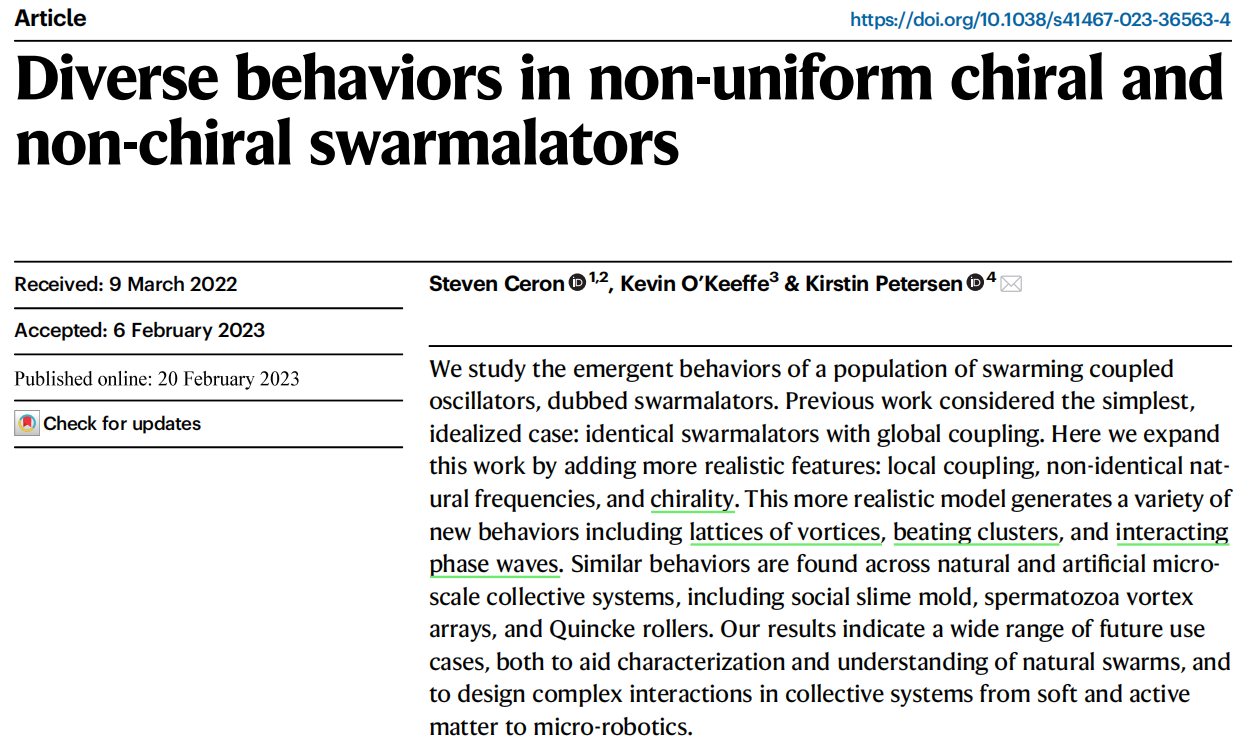
\includegraphics[width=\textwidth]{title.jpg}
    \end{figure}
\end{frame}

\begin{frame}
    In the original model:
    % 在原来的模型中,是把所有swarmalators的速度的模都设为一个常数,并且为0
        $$|\mathbf{v}_i|=v_0=0$$
    In this paper:
    % 在这篇paper中,作者做出了如下改进
        $$
        \mathbf{v}_i=c_i \mathbf{n}_i
        $$
    % 这么做的好处是速度与swarmalators的相位构成了一个直接映射,并且速度会像相位一样沿着圆形轨道的方向
        $$
        \begin{array}{c}
            c_i=\omega _iR_i\\
            \mathbf{n}_i=\left[ \begin{array}{c}
            \cos \left( \theta _i+\frac{\pi}{2} \right)\\
            \sin \left( \theta _i+\frac{\pi}{2} \right)\\
        \end{array} \right]\\
        \end{array}
        $$
    % 这里c_i依赖与自然频率吧omega_i和旋转半径R_i, n_i是一个单位向量,与相位角垂直,也就是说每个swarmalators的相位是它所在轨道上的角位置

\end{frame}

\begin{frame}
    New phase offset terms, $Q_{\dot{x}}$, $Q_{\dot{\theta}}$, which enable ‘frequency coupling’.
    % 文章还定义了新的相位偏移项,出发点是增加相反符号的自然品种的swarmalators之间的吸引力
    $$
    \begin{array}{c}
        Q_{\dot{x}}=\frac{\pi}{2}\left| \frac{\omega _j}{\left| \omega _j \right|}-\frac{\omega _i}{\left| \omega _i \right|} \right|\\
        Q_{\dot{\theta}}=\frac{\pi}{4}\left| \frac{\omega _j}{\left| \omega _j \right|}-\frac{\omega _i}{\left| \omega _i \right|} \right|\\
    \end{array}
    $$
    My understanding: 
    $$
    \begin{array}{c}
    Q_{\dot{x}}=\frac{\pi}{2}\left| \operatorname{sgn} \omega _j-\operatorname{sgn} \omega _i \right|=\begin{cases}
    \pi ,&		\operatorname{sgn} \omega _j\ne\operatorname{sgn} \omega _i\\
    0,&		\operatorname{sgn} \omega _j= \operatorname{sgn} \omega _i\\
    \end{cases}\\
    J\cos \left( \theta _j-\theta _i-Q_{\dot{x}} \right) =\begin{cases}
    -J\cos \left( \theta _j-\theta _i \right) ,&		Q_{\dot{x}}=\pi\\
    J\cos \left( \theta _j-\theta _i \right) ,&		Q_{\dot{x}}=0\\
    \end{cases}\\
    \end{array}
    $$
    
    
\end{frame}

\begin{frame}
    $$
    \dot{\mathbf{x}}_i=\mathbf{v}_i+\frac{1}{N}\sum_{j\ne i}^N{\left[ \frac{\mathbf{x}_j-\mathbf{x}_i}{\left| \mathbf{x}_j-\mathbf{x}_i \right|}\left( A+J\cos \left( \theta _j-\theta _i-Q_{\dot{x}} \right) \right) -B\frac{\mathbf{x}_j-\mathbf{x}_i}{\left| \mathbf{x}_j-\mathbf{x}_i \right|^2} \right]}
    $$

    $$
    J\cos \left( \theta _j-\theta _i-Q_{\dot{x}} \right) =\begin{cases}
        -J\cos \left( \theta _j-\theta _i \right) ,&		\operatorname{sgn} \omega _j\ne\operatorname{sgn} \omega _i\\
        J\cos \left( \theta _j-\theta _i \right) ,&		\operatorname{sgn} \omega _j= \operatorname{sgn} \omega _i\\
    \end{cases}
    $$
    \newline

    How can I ensure that $J\cos \left( \theta _j-\theta _i \right) > 0$, which means $\theta _j-\theta _i > \pi$ when $\operatorname{sgn} \omega _j\ne\operatorname{sgn} \omega _i$?
\end{frame}

% -----------------------------------------------------------------------------
\end{document}

